\section{Análisis exploratorio}

El análisis exploratorio se orienta a comprender la calidad y utilidad de los datos para el problema, no a producir visualizaciones sin propósito. La línea base identifica ausencia de valores nulos, 723 duplicados exactos, balance relativo de \texttt{target}, distribución observada de \texttt{sex} y edad entre 29 y 77 años.

\subsection{Efecto de la deduplicación}

Se comparó el archivo original con la versión deduplicada de 302 registros. El \tabref{tab:comparacion-target-sex} cuantifica las diferencias en puntos porcentuales, en lugar de asumir que la eliminación de duplicados no afecta las distribuciones. La proporción de \texttt{target}=1 aumenta 2,99 puntos porcentuales tras deduplicar; la distribución de \texttt{sex} cambia 1,35 puntos porcentuales por código.

\begin{table}[H]
  \centering
  \caption{Distribución de \texttt{target} y \texttt{sex}: original versus deduplicado}
  \label{tab:comparacion-target-sex}
  \begin{tabular}{lrrr}
    \toprule
    Categoría & Original (\%) & Deduplicado (\%) & Diferencia (pp) \\
    \midrule
    \texttt{target}=0 & 48,68 & 45,70 & -2,99 \\
    \texttt{target}=1 & 51,32 & 54,30 & +2,99 \\
    \texttt{sex}=0 & 30,44 & 31,79 & +1,35 \\
    \texttt{sex}=1 & 69,56 & 68,21 & -1,35 \\
    \bottomrule
  \end{tabular}
\end{table}

\begin{figure}[H]
  \centering
  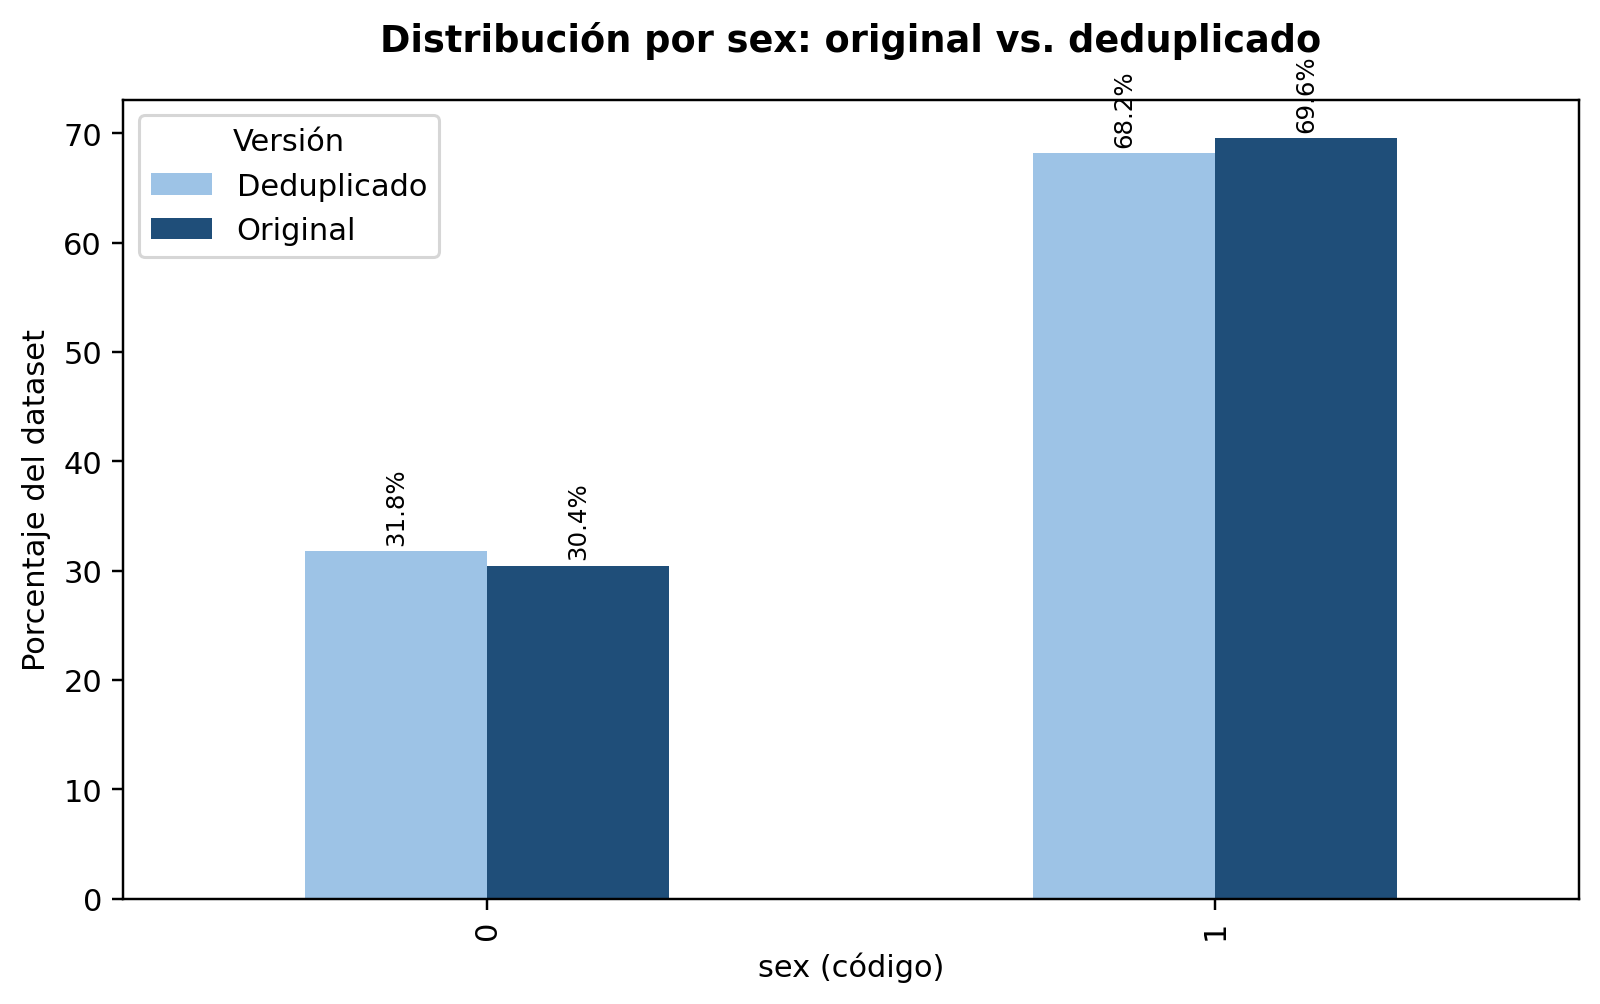
\includegraphics[width=0.82\textwidth]{../outputs/figures/comparacion_original_vs_unicos_sex.png}
  \caption{Comparación de la distribución de \texttt{sex} en el dataset original y deduplicado.}
  \label{fig:comparacion-sex}
\end{figure}

\begin{table}[H]
  \centering
  \caption{Distribución por rangos etarios: original versus deduplicado}
  \label{tab:comparacion-edad}
  \begin{tabular}{lrrr}
    \toprule
    Rango etario & Original (\%) & Deduplicado (\%) & Diferencia (pp) \\
    \midrule
    $<40$ & 5,56 & 4,97 & -0,59 \\
    40--49 & 23,12 & 23,84 & +0,72 \\
    50--59 & 41,17 & 41,39 & +0,22 \\
    60--69 & 26,83 & 26,49 & -0,34 \\
    70+ & 3,32 & 3,31 & -0,01 \\
    \bottomrule
  \end{tabular}
\end{table}

\begin{figure}[H]
  \centering
  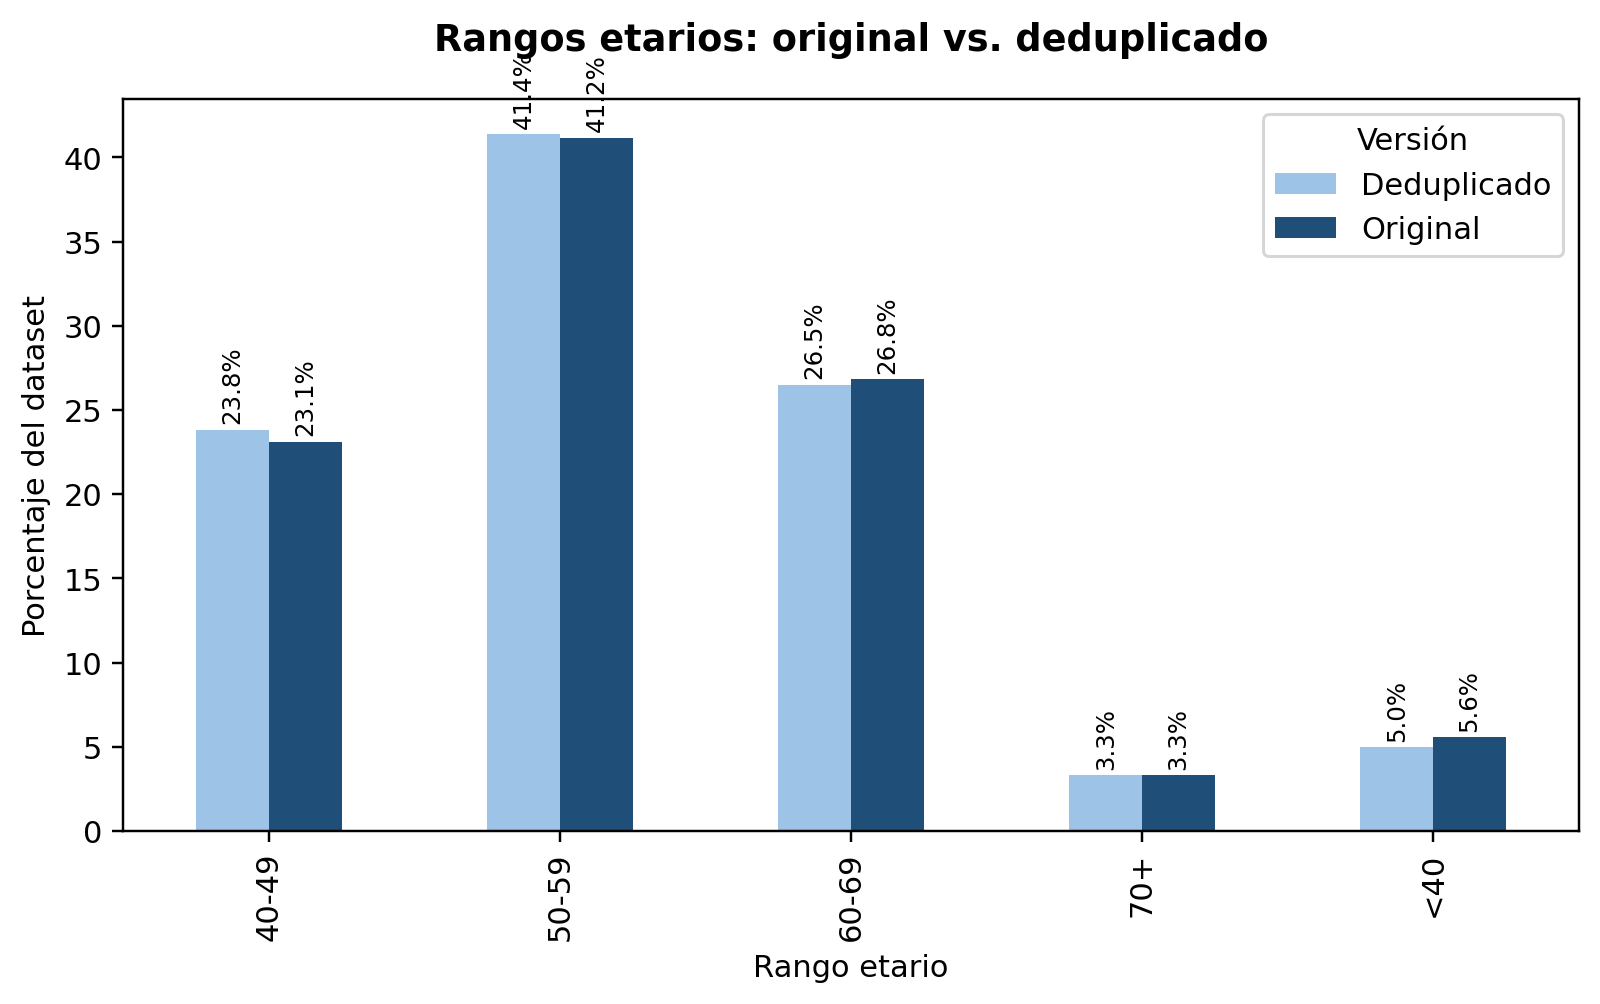
\includegraphics[width=0.82\textwidth]{../outputs/figures/comparacion_original_vs_unicos_edad.png}
  \caption{Comparación de los rangos etarios en el dataset original y deduplicado.}
  \label{fig:comparacion-edad}
\end{figure}

\subsection{Representación y subgrupos}

En la versión deduplicada, \texttt{sex}=0 concentra 96 registros (31,79\%) y \texttt{sex}=1 concentra 206 (68,21\%). Los rangos $<40$ (15 registros; 4,97\%) y 70+ (10; 3,31\%) disponen de menos evidencia que los rangos centrales. La \figref{fig:subgrupos-sex-edad} presenta los tamaños de las combinaciones \texttt{sex}$\times$rango etario. Los subgrupos \texttt{sex}=0 con $<40$ y con 70+ tienen cinco registros únicos cada uno; por ello, sus porcentajes de \texttt{target} son descriptivos y no constituyen evidencia de diferencias ni de sesgo demostrado.

\begin{figure}[H]
  \centering
  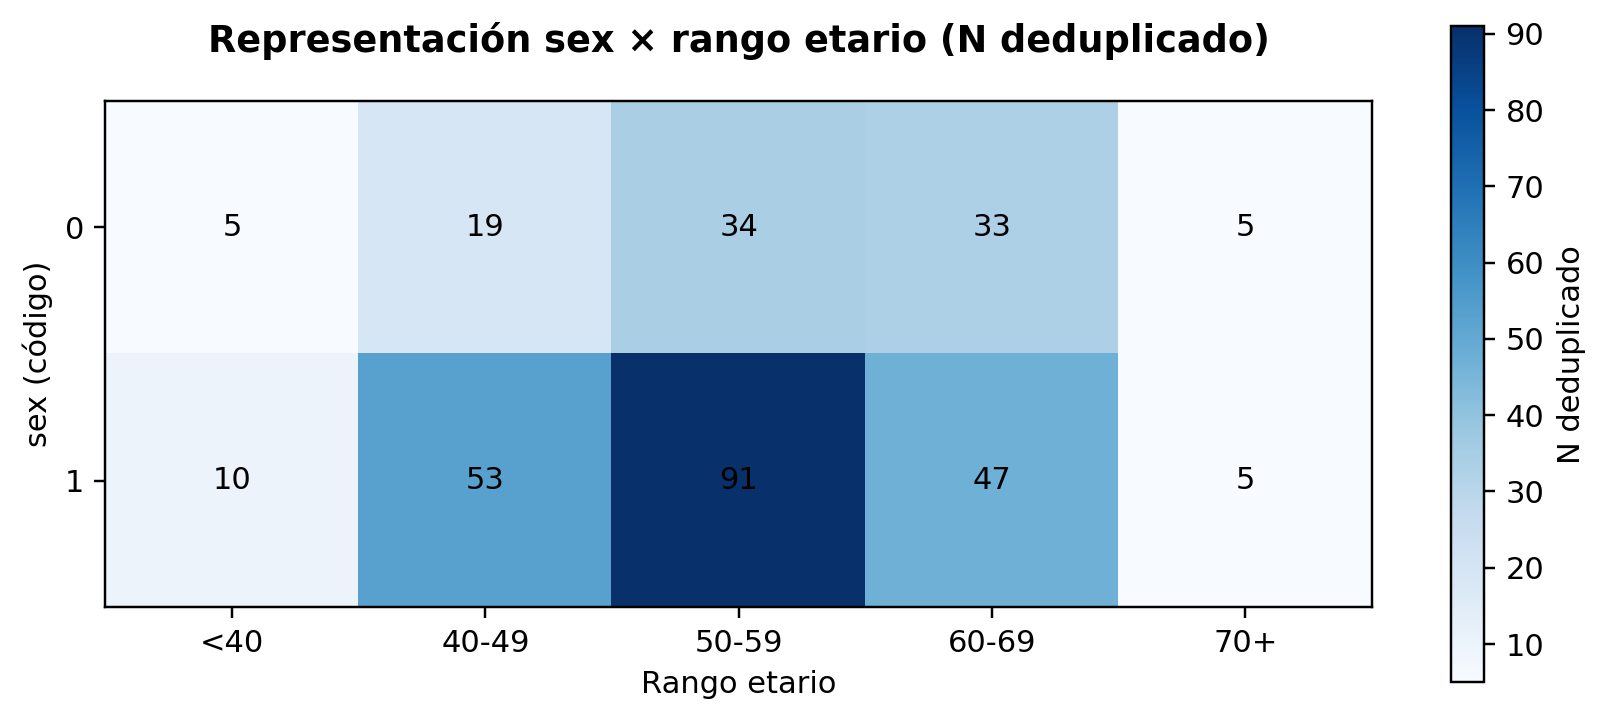
\includegraphics[width=0.88\textwidth]{../outputs/figures/representacion_sex_x_edad.png}
  \caption{Tamaño deduplicado de los subgrupos \texttt{sex}$\times$rango etario.}
  \label{fig:subgrupos-sex-edad}
\end{figure}

La evidencia sugiere posibles limitaciones de cobertura y generalización que deben validarse frente a la población objetivo. No permite afirmar discriminación, ni interpretar los códigos de \texttt{sex} sin confirmar su definición en la fuente oficial.
